\chapter{外部トリガを用いた応答評価試験}
この章では,外部トリガを用いた粒子線に対する応答評価試験について述べる.\ref{sec:extplan}節で外部トリガを用いた応答評価試験の概要,\ref{sec:extsetup}節で外部トリガでデータ取得をする際のセットアップ,\ref{sec:exthow}節で手順,\ref{sec:extconc}節で取得データ結果を示し,\ref{sec:selfsum}節で考察を行なっている.

\section{外部トリガを用いた応答評価試験概要}
\label{sec:extplan}
この節では,Quad Chip RD53Aモジュールに対して行われる品質試験について述べる.\ref{sec:masspro}節で述べたように,現在実機で用いるモジュールを量産するための準備として,プロトタイプ版のASICが4 $\mathrm{Chip}$搭載されたQuad Chip RD53Aモジュールで量産体制の確認が計画されている.この時に,バンプボンディングに異常が無いかを確認するための試験が,外部トリガを用いた応答評価試験である.現在計画されている試験は,クーリングボックスと呼ばれる,温度が低温に維持された小さな箱の中で行い,トリガには前章で述べたHitOR信号ではなく,トリガシンチの信号を外部トリガとして用いる.トリガシンチの構成については\ref{sec:extsetup}節で詳しく述べる.計画されている外部トリガを用いた応答評価試験セットアップを図\ref{fig:trigplan}に示す.

\begin{figure}[h]
  \centering
  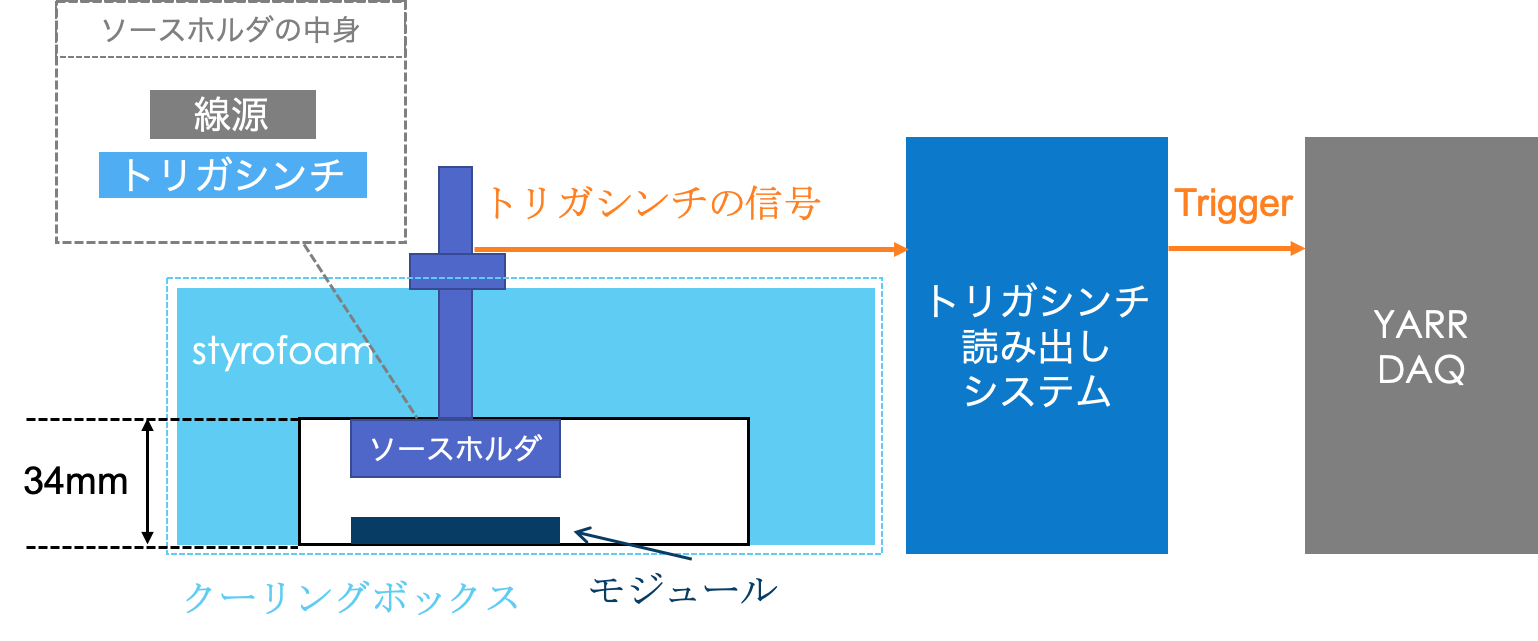
\includegraphics[width=15cm]{./figure/trigplan.png}
  \caption{計画されている外部トリガを用いた応答評価試験セットアップ}
  \label{fig:trigplan}
\end{figure}

計画されているセットアップに近付けるようにして以降,外部トリガを用いた応答評価試験を行なった.

%線源とモジュールの間にシンチレータを配置し,そのシンチレータに粒子が入射した時の発光をMPPCで検出し信号として読み出すことで,トリガに用いる.このシンチレータとMPPCが合わさったものを以降トリガシンチと呼ぶ.トリガシンチは非常にコンパクトな環境で用いられることや,線源とモジュールの間に配置されることから,なるべく小さく,粒子線を遮ることのないように薄くあることが要求されている.このセットアップで可能な外部トリガを用いた応答評価試験の手法を考えた.


\section{外部トリガを用いた応答評価試験セットアップ}
\label{sec:extsetup}
今回行なった外部トリガを用いた応答評価試験のセットアップを図\ref{fig:extsetup}に示す.主にセルフトリガの際と変わらず,RD53A搭載のSingle Chip Card(SCC)とFPGAボード,PCを用いて読み出しシステムを構成している.読み出しASICとFPGAボードは,FMC-mDP変換ボードを用いてケーブルにて接続を行い,FPGA内部でASICからのデータ信号の処理を行なった.また,高速通信用インターフェースでPCとFPGAボードを接続し,データ転送を行なった.そして,これらに加え,今回は外部トリガにトリガシンチを用いるため,トリガシンチ,トリガシンチ信号読み出しシステム,ソースホルダが存在する.トリガシンチ信号読み出しシステムのDPコネクタとアダプタカードのport Dが繋げられている.\par

\begin{figure}[h]
  \centering
  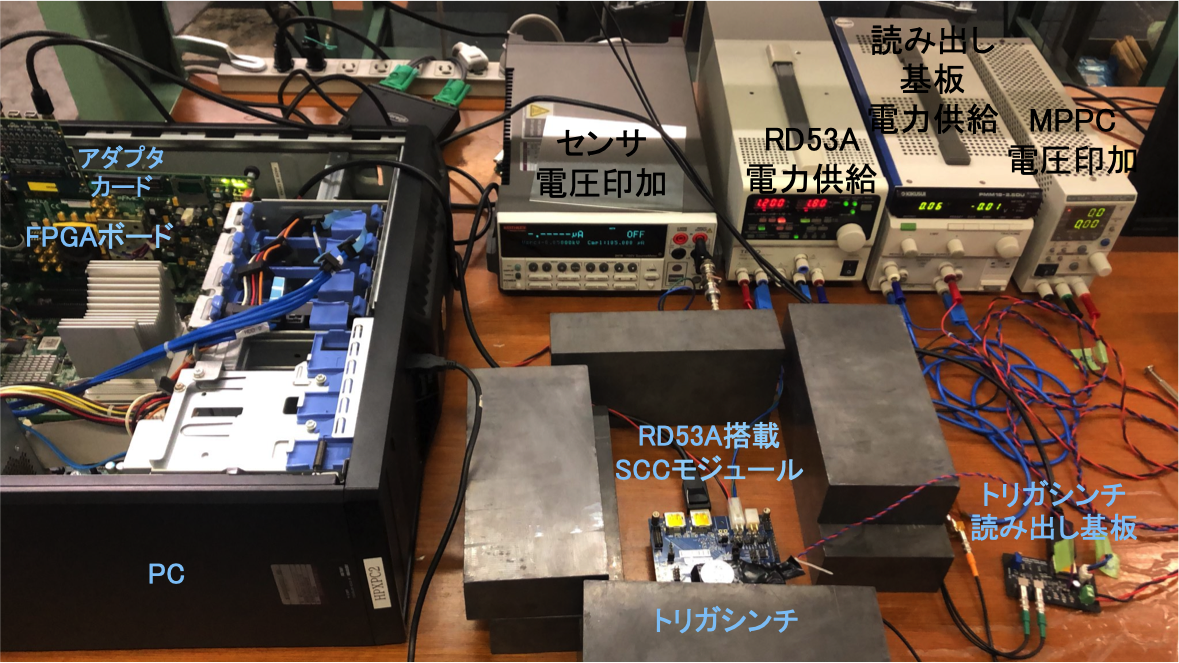
\includegraphics[width=15cm]{./figure/extsetup.png}
  \caption{セットアップの様子}
  \label{fig:extsetup}
\end{figure}

\subsection{トリガシンチ}
今回トリガシンチに使用したシンチレータと,MPPCをシンチレータに取り付けた様子を図\ref{fig:scin}に示す.図中のライトガイドとは,シンチレータに粒子が入射した時に発光した光を効率よくMPPCまで伝えるための部品である.また,\ref{sec:trigplan}でも述べたように,非常にコンパクトな環境での利用を目的としているため,トリガシンチは箱の中,読み出し回路は箱の外で使用される.それに伴って,MPPCの足は約30 $\mathrm{cm}$のケーブルをはんだづけすることで延長し,トリガシンチの信号を箱の外まで伝えられるようにしてある.また,荷電粒子がトリガシンチに遮蔽され,モジュールまで届かなくなることがないように,シンチレータは0.5 $\mathrm{mm}$と非常に薄いものを使用している.シンチレータは光収集率をよくするために,白い紙で覆ったのち,MPPCと共に黒テープで遮光を行なった.その様子を図\ref{fig:trigscin1}に示す.トリガシンチを構成する要素えあるMPPCとシンチレータについて以降述べる.

\begin{figure}[h]
  \centering
  \begin{minipage}[b]{0.45\linewidth}
    \centering
    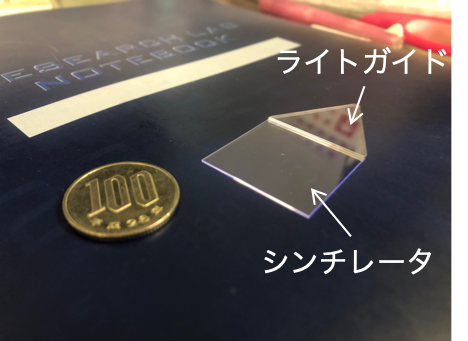
\includegraphics[width=6cm]{./figure/trigscin.png}
    \subcaption{使用したシンチレータとライトガイド}
    \label{fig:scin}
  \end{minipage}
  \begin{minipage}[b]{0.45\linewidth}
    \centering
    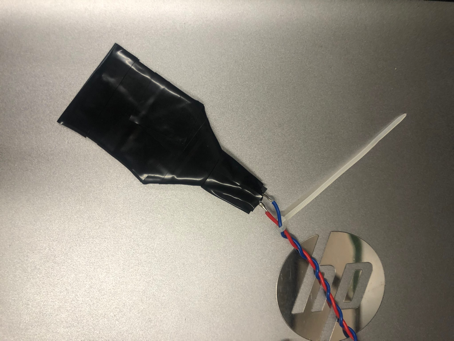
\includegraphics[width=6cm]{./figure/trigscin1.png}
    \subcaption{MPPCを取り付け,遮光したトリガシンチ}
    \label{fig:trigscin}
  \end{minipage}
  \caption{0.5mmのシンチレータの様子}
  \label{fig:trigscin1}
\end{figure}


\subsubsection*{MPPC}
MPPCとは,Silicon Photomultipliers(SiPM)と呼ばれるデバイスの一種であり,複数の半導体光検出器・アバランシェフォトダイオード(APD)から成るフォトンカウンティングデバイスである.本論文で用いたMPPC・HAMAMATSU S13360-1325CSは,$1.3 \times 1.3 \mathrm{mm^2}$の受光面に$25 \times 25 \mathrm{\mu m^2}$のAPDが敷き詰められている.MPPCの構成を図\ref{fig:APD}に示す.

\begin{figure}[h]
  \centering
  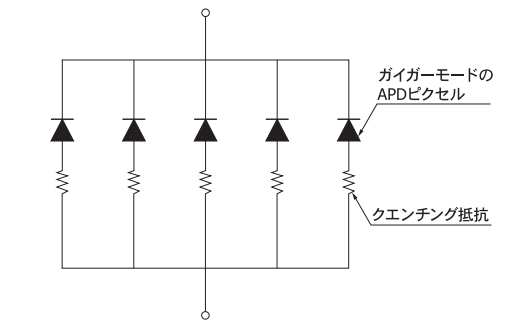
\includegraphics[width=8cm]{./figure/apd.png}
  \caption{MPPCの構成\cite{03handbo69:online}}
  \label{fig:APD}
\end{figure}

全てのAPDの読み出し線,および電圧供給の線は共通していて,全てのAPDピクセルからのシグナルの総和が1つのMPPCからの出力として得られる構造になる.MPPCでは各APDピクセルからの応答が良く揃っているために、総和として出力されるシグナル$Q_{total}$は式\ref{eq:photon}で示されるように光子を受光したピクセル数$N$に1つのAPDから得られるシグナル$Q$をかけた値となる

\begin{eqnarray}
  Q_{total} = N \times Q
\end{eqnarray}

受光したピクセル数は、光が微弱である時入射する光量に比例するため, MPPCは非常に高いフォトンカウンティング能力を備えている.

\subsubsection*{シンチレータ}
シンチレータとは,放射線のエネルギーを吸収し,内部で励起あるいは電離が起こることで発光する物質である.材質には,無機結晶や液体など様々あるが,本論文では,プラスチックシンチレータを用いた.

\subsection{トリガシンチの信号読み出しシステム}
本研究を行うにあたって,MPPCからの信号をYARRのDAQシステムのトリガとして使用できるように波形整形できるシステムを作成した.システムの全体像を図\ref{fig:exttriggersetup}に示し,各回路の役割とトリガシンチの信号がどのように伝達されるかを図\ref{fig:exttriggersignal}に示す.トリガシンチの信号は読み出し基板1で増幅され,コンパレータによってアナログデジタル変換される.その後,ATLYSにてDelayされ,読み出し基板2によってTTLからLVDS変換され,DPコネクタから信号が出力される仕組みである.読み出し基板にDelay機能が実装されていないため,このように2枚の読み出し基板とFPGAボードで構成されている.

\begin{figure}[h]
  \centering
  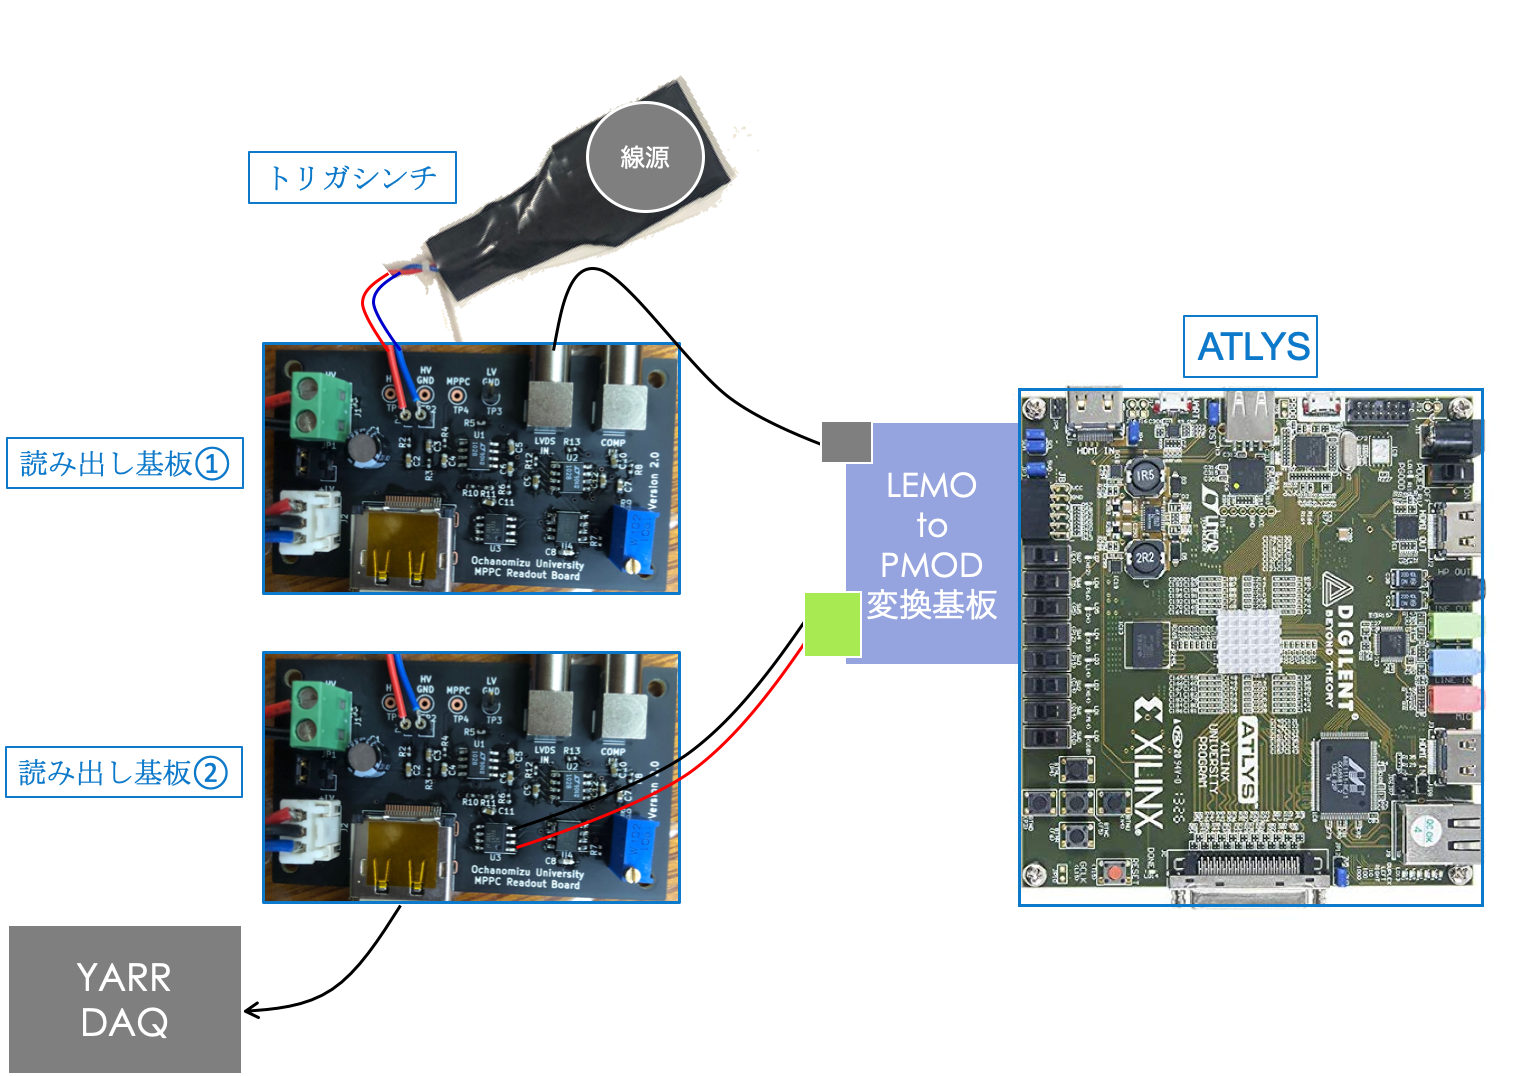
\includegraphics[width=15cm]{./figure/exttriggersetup.png}
  \caption{トリガシンチの信号を読み出すシステム全体像}
  \label{fig:exttriggersetup}
\end{figure}

\begin{figure}[h]
  \centering
  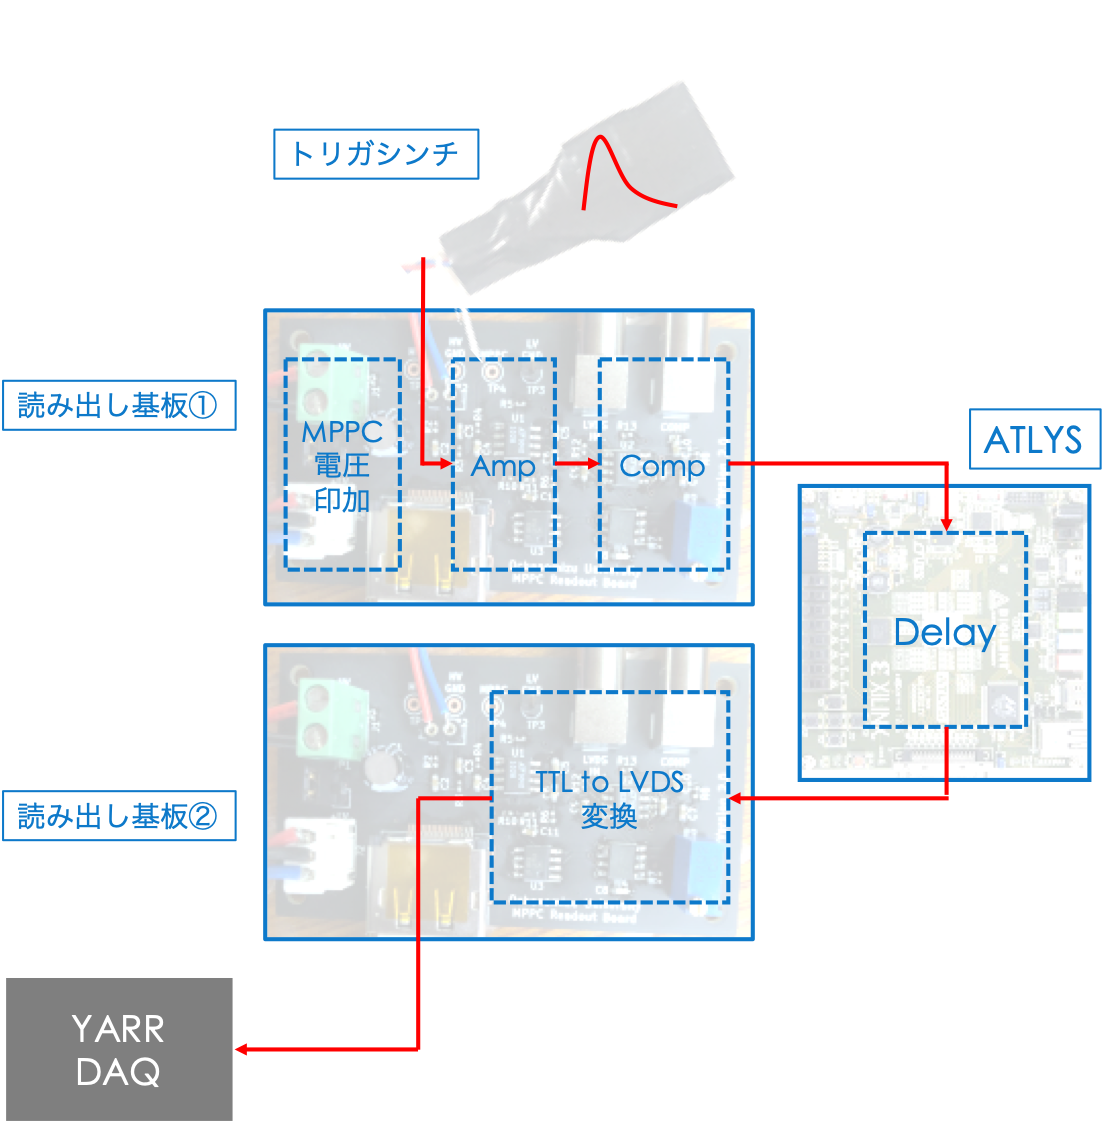
\includegraphics[width=10cm]{./figure/exttriggersignal.png}
  \caption{トリガシンチの信号がYARR-DAQに伝わるまでの様子}
  \label{fig:exttriggersignal}
\end{figure}

\subsubsection*{読み出し基板1,2}
本研究を行うにあたって,MPPCからの信号を波形整形する基板を作成した.基板を図\ref{fig:pcb}に示す.主に,電圧供給回路,反転増幅回路,コンパレータ回路,LVDS変換回路から構成されている.基板はKiCADというCERN開発のオープンソースプリント基板CADを用いて設計・作成した.LEMO1からは増幅されたMPPCのアナログ信号を,LEMO2からはコンパレータによって閾値電圧と比較することで変換されたデジタル信号を,DPからはTTLだったデジタル信号が変換されてLVDS出力のデジタル信号を読み出すことができる.その3点についてオシロスコープで観測した波形を図\ref{fig:extosiro}に示す.トリガシンチに荷電粒子が入射した信号を得たいため,オシロスコープの様子から,コンパレータの比較電圧は75 $\mathrm{mV}$とした.

\begin{figure}[h]
  \centering
  \begin{minipage}[b]{0.45\linewidth}
    \centering
    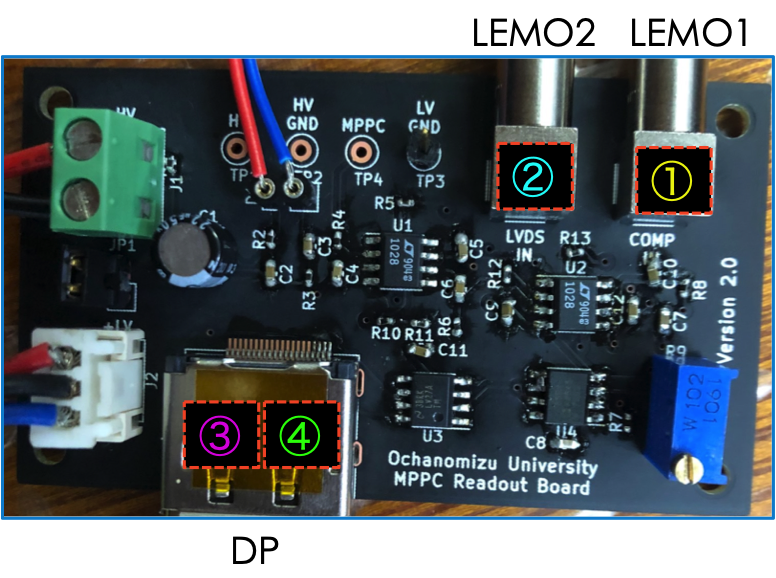
\includegraphics[width=7cm]{./figure/pcb.png}
    \subcaption{基板の様子}
    \label{fig:pcb}
  \end{minipage}
  \begin{minipage}[b]{0.45\linewidth}
    \centering
    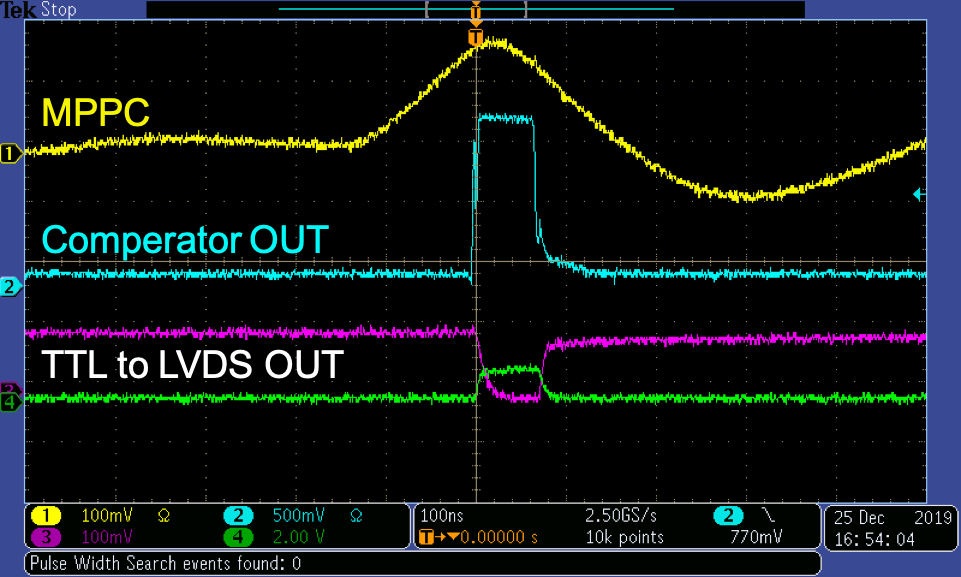
\includegraphics[width=8cm]{./figure/pcbosiro.png}
    \subcaption{動作確認したオシロスコープの様子}
    \label{fig:extosiro}
  \end{minipage}
  \caption{トリガシンチの信号を波形整形する基板}
\end{figure}

\subsubsection*{ATLYS}
Delay機能が実装されたXilinx, Inc. の spaltan6 FPGA搭載ATLYS評価ボードを使用した.124 $\mathrm{nsec}$Delayさせるように設定した.

\subsection{ソースホルダ}
ソースホルダの外観を図\ref{fig:sourceholder}に示す.クーリングボックス内で使用することを想定し,コンパクトな作りになっている.これは,FreeCADというオープンソース汎用3D CADモデラで設計し,3Dプリンタを用いて作成した.ソースホルダは箱,蓋,軸,留め具の4パーツに分かれていて,蓋の部分には線源を固定するための窪みが存在する.

\begin{figure}[h]
  \centering
  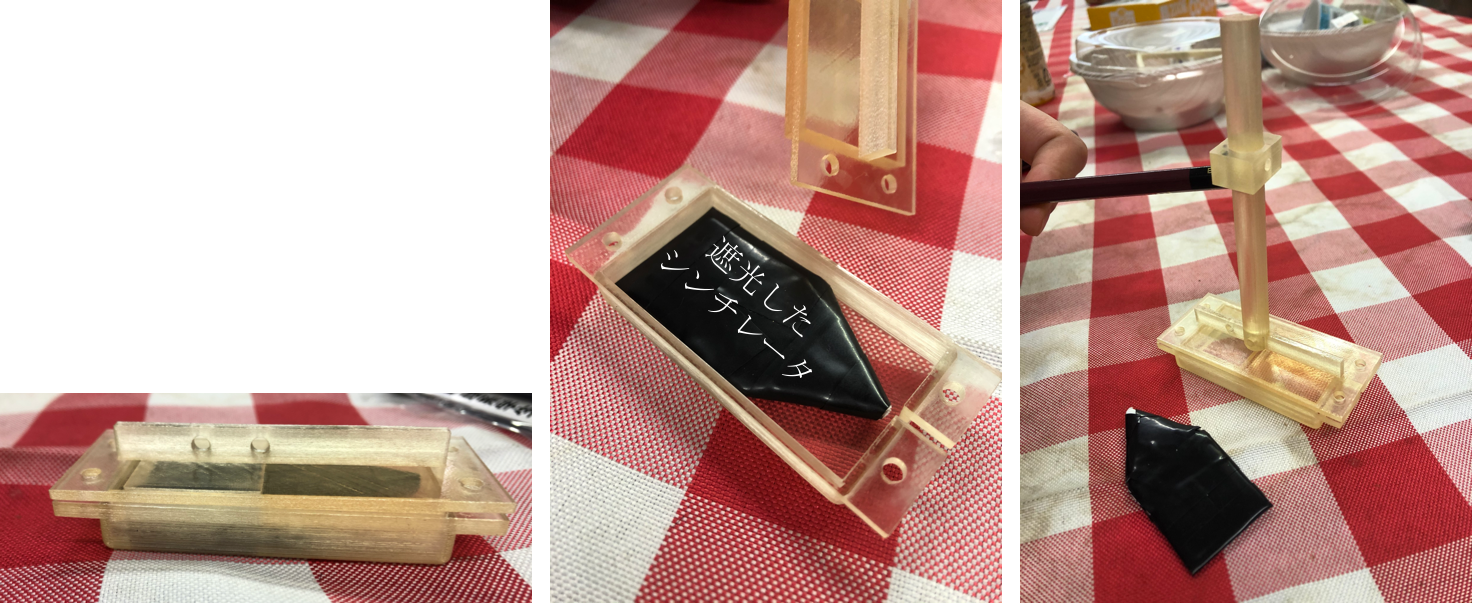
\includegraphics[width=15cm]{./figure/sourceholder.png}
  \caption{ソースホルダの様子}
  \label{fig:sourceholder}
\end{figure}


\section{応答評価試験手順}
\label{sec:exthow}
まず,前章で述べたようなトリガシンチの信号がFPGAまで伝達され,処理されているかの確認を行った.その確認の様子を図に\ref{fig:extwf}に示す.

\begin{figure}[h]
  \centering
  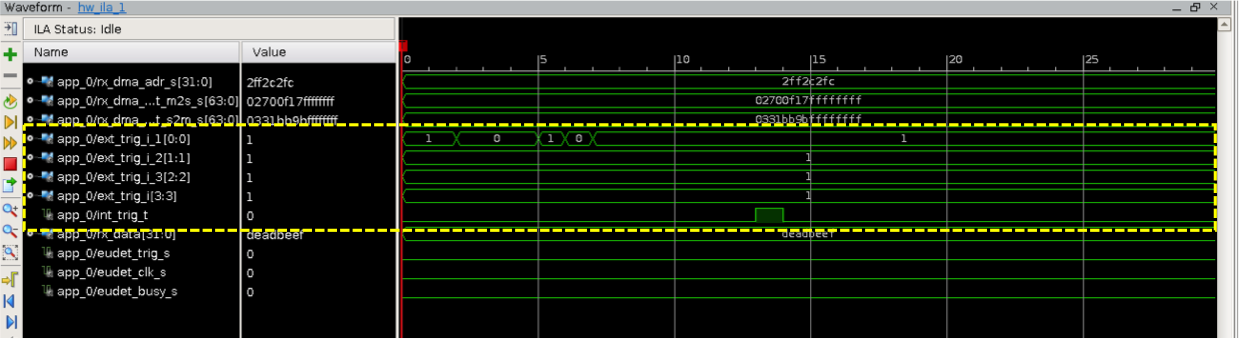
\includegraphics[width=17cm]{./figure/extWF.png}
  \label{fig:extwf}
  \caption{VivadoのLogic Analyzerでトリガシンチからの信号を確認した様子}
\end{figure}

今回は''ext\_trig\_i[0:0]''にのみ信号を入力しているため,その部分のみが0から1へと変化している.また,''int\_trig''も0から1に変化していることから,ファームウェアにてトリガシンチの信号の受信・処理が正常に行われていることが確認できる.\par
次に,Latency Scanを行なった.Latency Scanの結果を図\ref{fig:exttriglatency}に示す.この結果より,''LatencyConfig''値を211に設定することで,Latencyを合わせた.
\begin{figure}[h]
  \centering
  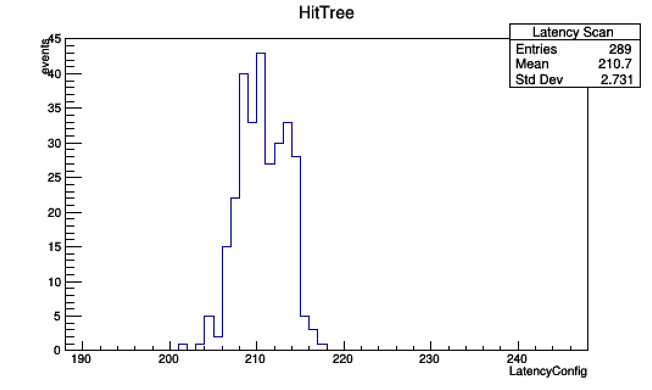
\includegraphics[width=14cm]{./figure/latencydist.png}
  \caption{''LatencyConfig''値とL1ID $== 7$だったイベント数の関係}
  \label{fig:exttriglatency}
\end{figure}

Latencyを合わせた上で,トリガシンチの上に線源を設置した場合としない場合それぞれについて,30分間の外部トリガによるデータ取得を行なった.

\section{応答評価試験結果}
\label{sec:extconc}
表\ref{tab:ext}と図\ref{fig:ext}に線源をトリガシンチの上に設置した場合としない場合それぞれの,30分間の外部トリガによるデータ取得結果を示す.
\begin{table}[h]
  \centering
  \caption{線源の有無それぞれのヒットレート}
  \begin{tabular} {|l|c|c||c|} \hline
     & \# Hit & 時間[s] & Hitレート[hits/sec] \\  \hline
    線源なし & $3.528 \times 10^6$ & 1800 & 1960 \\ 
    線源あり & $3.599 \times 10^6$ & 1800 & 2000 \\ \hline
  \end{tabular}
  \label{tab:ext}
\end{table}

\begin{figure}[h]
  \centering
  \begin{minipage}[b]{0.45\linewidth}
    \centering
    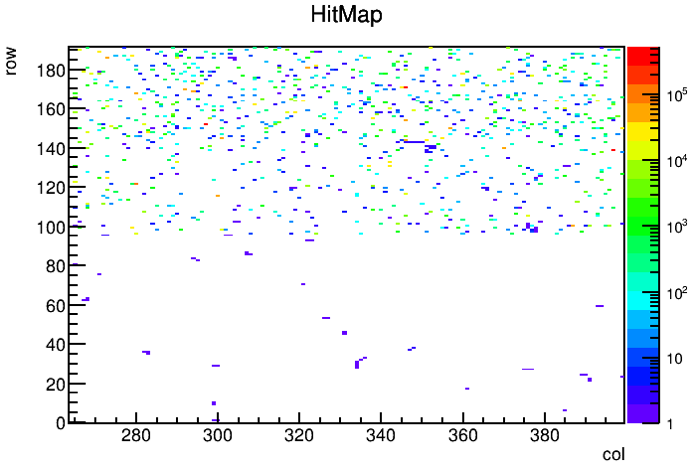
\includegraphics[width=7cm]{./figure/selftrigwo.png}
    \subcaption{線源を置かない場合}
    \label{fig:extwo}
  \end{minipage}
  \begin{minipage}[b]{0.45\linewidth}
    \centering
    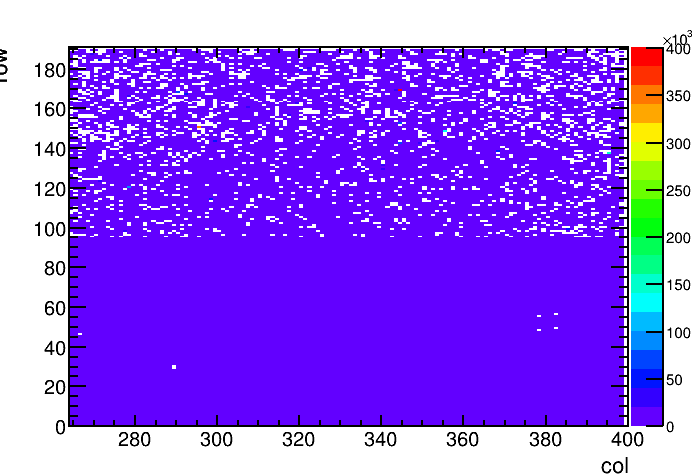
\includegraphics[width=7cm]{./figure/selftrigw.png}
    \subcaption{線源を置いた場合}
    \label{fig:extw}
  \end{minipage}
  \caption{ヒットの分布}
  \label{fig:ext}
\end{figure}

\section{考察}
\label{sec:extsum}

%
%\subsection*{MPPC}
%MPPCとは,Silicon Photomultipliers(SiPM)と呼ばれるデバイスの一種であり,複数の半導体光検出器・アバランシェフォトダイオード(APD)から成るフォトンカウンティングデバイスである.本論文で用いたMPPC・HAMAMATSU S13360-1325CSは,$1.3 \times 1.3 \mathrm{mm^2}$の受光面に$25 \times 25 \mathrm{\mu m^2}$のAPDが敷き詰められている.MPPCの構成を図\ref{fig:APD}に示す.
%
%\begin{figure}[h]
%  \centering
%  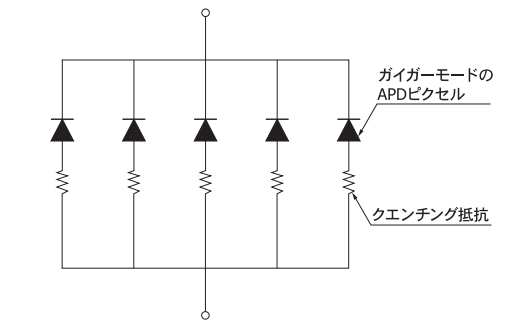
\includegraphics[width=8cm]{./figure/apd.png}
%  \caption{MPPCの構成\cite{03handbo69:online}}
%  \label{fig:APD}
%\end{figure}
%
%全てのAPDの読み出し線,および電圧供給の線は共通していて,全てのAPDピクセルからのシグナルの総和が1つのMPPCからの出力として得られる構造になる.MPPCでは各APDピクセルからの応答が良く揃っているために、総和として出力されるシグナル$Q_{total}$は式\ref{eq:photon}で示されるように光子を受光したピクセル数$N$に1つのAPDから得られるシグナル$Q$をかけた値となる
%
%\begin{eqnarray}
%  Q_{total} = N \times Q
%\end{eqnarray}
%
%受光したピクセル数は、光が微弱である時入射する光量に比例するため, MPPCは非常に高いフォトンカウンティング能力を備えている.
%
%\subsection*{シンチレータ}
%シンチレータとは,放射線のエネルギーを吸収し,内部で励起あるいは電離が起こることで発光する物質である.材質には,無機結晶や液体など様々あるが,本論文では,プラスチックシンチレータを用いた.
%
%\section{トリガシンチの基礎測定}
%この節では,RD53Aに対して行われる品質試験で外部トリガとして使用されるトリガシンチの性能の基礎測定について述べる.
%
%\subsection{概要}
%今回使用したシンチレータと,光を読み出すためにMPPCをシンチレータに取り付けた様子を図\ref{fig:scin}に示す.図中のライトガイドとは,シンチレータに粒子が入射した時に発光した光を効率よくMPPCまで伝えるための部品である.また,\ref{sec:trigplan}でも述べたように,非常にコンパクトな環境での利用を目的としているため,トリガシンチは箱の中,読み出し回路は箱の外で使用される.そのため,MPPCの足は約30 $\mathrm{cm}$のケーブルをはんだづけすることで延長し,MPPCからの信号を箱の外まで伝えられるようにしてある.シンチレータは0.5 $\mathrm{mm}$と非常に薄いものを使用し,MPPCと共に黒テープで遮光を行なった.
%
%\begin{figure}[h]
%  \centering
%  \begin{minipage}[b]{0.45\linewidth}
%    \centering
%    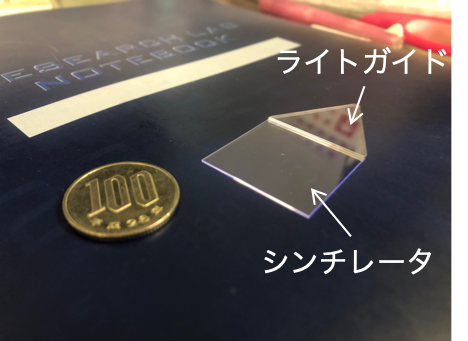
\includegraphics[width=6cm]{./figure/trigscin.png}
%    \subcaption{使用したシンチレータとライトガイド}
%    \label{fig:scin}
%  \end{minipage}
%  \begin{minipage}[b]{0.45\linewidth}
%    \centering
%    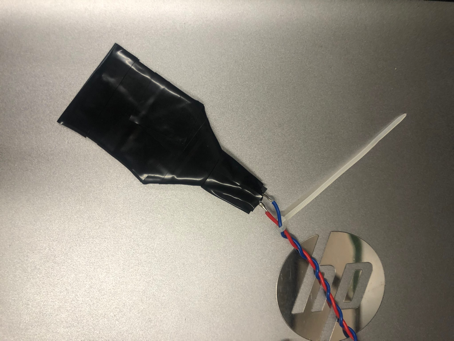
\includegraphics[width=6cm]{./figure/trigscin1.png}
%    \subcaption{MPPCを取り付け,遮光したトリガシンチ}
%    \label{fig:trigscin}
%  \end{minipage}
%  \caption{0.5mmのシンチレータの様子}
%  \label{fig:trigscin1}
%\end{figure}
%
%
%このトリガシンチに対して以下の2点に関する基礎測定を行なった.
%\begin{itemize}
%\item 線源を置いた時と置かない時のトリガレート 
%\item MPPCが読み出した光量と粒子線が入射した位置の依存性
%\end{itemize}
%
%また,今回は使用が予定されている環境がコンパクトな環境なため,ライトガイドを用いた場合と用いなかった場合で,トリガレートや光量に差がないのであれば,ライトガイドはない方が望ましい.よって,ライトガイドが無い場合についても同様の点について基礎測定を行なった.
%
%\subsection{基礎測定のセットアップ}
%図\ref{fig:trigsetup}に読み出しシステムの概要を示す.主に,シンチレータとMPPC,読み出し基板,ADCモジュールで構成している.シンチレータで発光した光をMPPCで検出し,読み出し回路でデジタル信号として読み出す.読み出し基板とADCモジュールはコネクタを通してLEMOケーブルで接続している.
%
%\begin{figure}[h]
%  \centering
%  \includegraphics[width=15cm]{./figure/trigsetup.png}
%  \caption{トリガシンチの基礎測定セットアップ}
%  \label{fig:trigsetup}
%\end{figure}
%
%\subsubsection*{トリガシンチの信号を波形整形する基板}
%本研究を行うにあたって,MPPCからの信号を波形整形する基板を作成した.基板を図\ref{fig:extcircle}に示す.主に,電圧供給回路,反転増幅回路,コンパレータ回路,LVDS変換回路から構成されている.基板はKiCADというCERN開発のオープンソースプリント基板CADを用いて設計・作成した.LEMO1からは増幅されたMPPCのアナログ信号を,LEMO2からはコンパレータによって閾値電圧と比較することで変換されたデジタル信号を,DPからはTTLだったデジタル信号が変換されてLVDS出力のデジタル信号を読み出すことができる.その3点についてオシロスコープで観測した波形を図\ref{fig:extosiro}に示す.基礎測定では,LEMO2の出力からGATE信号を生成し,LEMO1の出力のデータを測定した.
%
%\begin{figure}[h]
%  \centering
%  \begin{minipage}[b]{0.45\linewidth}
%    \centering
%    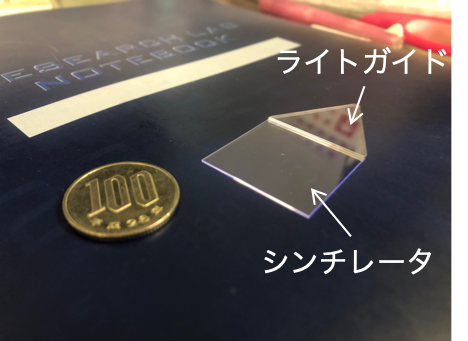
\includegraphics[width=6cm]{./figure/trigscin.png}
%    \subcaption{基板の様子}
%    \label{fig:pcb}
%  \end{minipage}
%  \begin{minipage}[b]{0.45\linewidth}
%    \centering
%    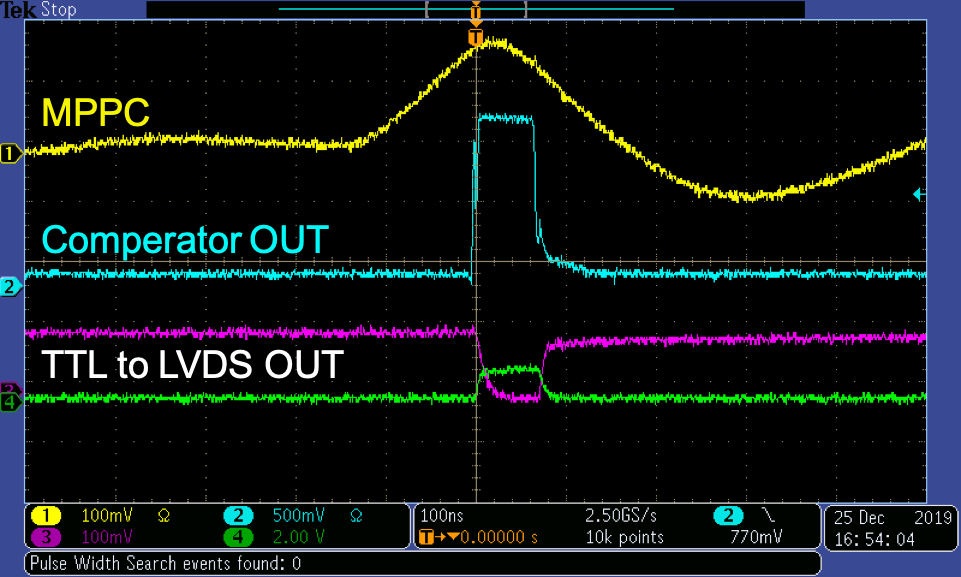
\includegraphics[width=8cm]{./figure/pcbosiro.png}
%    \subcaption{動作確認したオシロスコープの様子}
%    \label{fig:extosiro}
%  \end{minipage}
%  \caption{トリガシンチの信号を波形整形する基板}
%\end{figure}
%
%\subsection{光量と粒子の入射位置の依存性測定}
%粒子の入射位置がMPPCから最も離れている時と,最も近い時で,トリガシンチの読み出す光量にどれくらいの差が出るのかをライトガイドがある場合とない場合で測定した.ライトガイドの必要性を評価するためにこの測定を行なった.
%
%\subsubsection*{手順}
%測定を行なった時のトリガシンチと粒子の入射位置を図\ref{fig:trigscinlg}に示す.粒子の入射位置は,トリガシンチと線源の間に小さな穴の空いた鉄板を設置することで調節した.鉄板の穴の位置がMPPCから最も離れている時(図中A)と,最も近い時(図中B)で,トリガシンチから読み出された光量を測定した.ライトガイドありの場合となしの場合で,位置による光量の差に変化があるかを測定した.コンパレータの比較電圧$V_{ref}$を150 $\mathrm{mV}$に設定した.
%
%\begin{figure}[h]
%  \centering
%  \begin{minipage}[b]{0.45\linewidth}
%    \centering
%    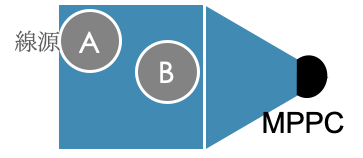
\includegraphics[height=2cm]{./figure/trigscinwlg.png}
%    \subcaption{ライトガイドがある場合}
%    \label{fig:trigscinwlg}
%  \end{minipage}
%  \begin{minipage}[b]{0.45\linewidth}
%    \centering
%    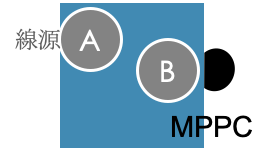
\includegraphics[height=2cm]{./figure/trigscinwolg.png}
%    \subcaption{ライトガイドがない場合}
%    \label{fig:trigscinwolg}
%  \end{minipage}
%  \caption{トリガシンチと粒子の入射位置の関係}
%  \label{fig:trigscinlg}
%\end{figure}
%
%\subsubsection*{結果}
%測定結果は図\ref{fig:trigscincon}のようになっている.
%
%\begin{figure}[h]
%  \centering
%  \begin{minipage}[b]{0.45\linewidth}
%    \centering
%    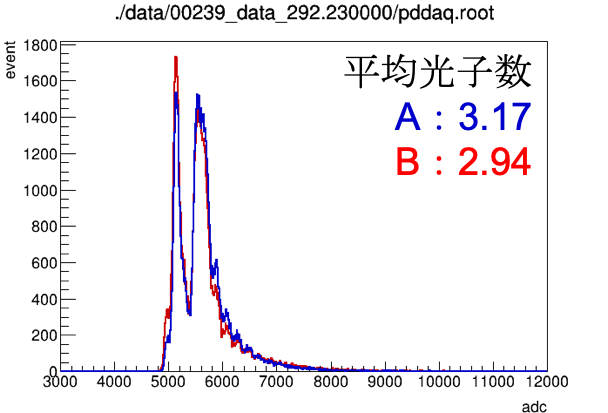
\includegraphics[width=7.5cm]{./figure/trigscinwlgcon.png}
%    \subcaption{ライトガイドがある場合}
%    \label{fig:trigscinwlg}
%  \end{minipage}
%  \begin{minipage}[b]{0.45\linewidth}
%    \centering
%    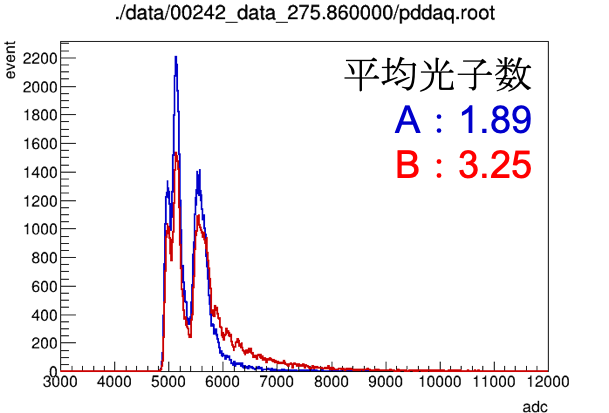
\includegraphics[width=7.5cm]{./figure/trigscinwolgcon.png}
%    \subcaption{ライトガイドがない場合}
%    \label{fig:trigscinwolg}
%  \end{minipage}
%  \caption{トリガシンチと粒子の入射位置の関係}
%  \label{fig:trigscinlgcon}
%\end{figure}
%
%
%
%\subsection{トリガレートの測定}
%トリガシンチの上に線源を配置した時としない時で,どれくらい
%\subsubsection*{手順}
%トリガシンチの上に線源を配置した時としない時で,100000イベントのデータを取得するのにかかる時間を測定した.
%
%\subsubsection*{結果}
%トリガシンチの上に線源を配置した時としない時のトリガレートの比較結果は表\ref{tab:trigscinrate}のようになっている.
%
%\
%
%
%
%\section{外部トリガを用いた応答評価試験セットアップ}
%\label{sec:extsetup}
%RD53Aの量産にあたって,行われる品質試験では,外部トリガを用いた応答評価試験が行われる.そのため,実際に行われる試験環境に近いセットアップで試験を行なった.セットアップの写真を以下に示す.MPPCには58$\mathrm{V}$印加した.SCCとFPGAボード,PCを用いてシステムを組む大枠は変わらずに,線源の配置とトリガに使用するものが異なっている.\par
%実際に行われる試験は,クーリングボックスと呼ばれる,温度が低温に維持された小さな箱の中で行い,トリガには前章で述べたHitOR信号ではなく,シンチレータからの光信号を用いる.シンチレータは線源とモジュールの間に設置するため,なるべく$\beta$線を遮らないように,厚みは0.5$\mathrm{mm}$と非常に薄いものを使用した.
%実際に行われる試験環境はクーリングボックスと呼ばれる,温度が低温に維持された小さな箱の中で行う.それに合う応答評価試験セットアップを考えるにあたって,線源とシンチレータ,シンチレータの光信号を電気信号に変換するMPPCが乗ったソースホルダと,MPPCからのアナログ信号を波形整形し,LVDSのデジタル信号に変換するような基板の設計を行なった.
%
%\subsection{ソースホルダの設計}
%ソースホルダの外観を以下に示す.クーリングボックス内で使用することを想定し,コンパクトな作りになっている.これは,FreeCADというオープンソース汎用3D CADモデラで設計し,3Dプリンタを用いて作成した.
%
%\subsection{MPPCからの信号を波形整形する回路}
%
%\subsubsection*{回路の動作確認}
%MPPCからの信号を正しく波形整形できているかをオシロスコープを用いて確認した.増幅されたMPPCからの信号がコンパレータによって,デジタル信号に変換され,TTL to LVDS変換のチップによって,差動信号に変換されている様子がわかる.
%
%\section{トリガシンチの基礎測定}
%この回路では,信号を出力をコンパレータの閾値によって設定している.この閾値によって,MPPCからの信号が削られることなく伝達されているかを確認した.
%
%\section{応答評価試験手順}
%\label{sec:exthow}
%\section{応答評価試験結果}
%\label{sec:extconc}
%\section{考察}
%\label{sec:extsum}
